In this section, CLIP with prompt engineering for animal action recognition has been explored to solve the long-tail issue, while AFRICAN has been proposed to deal with temporal redundancy. 

\section{CLIP with Prompt Engineering}

\begin{figure}[ht]
    \centering
    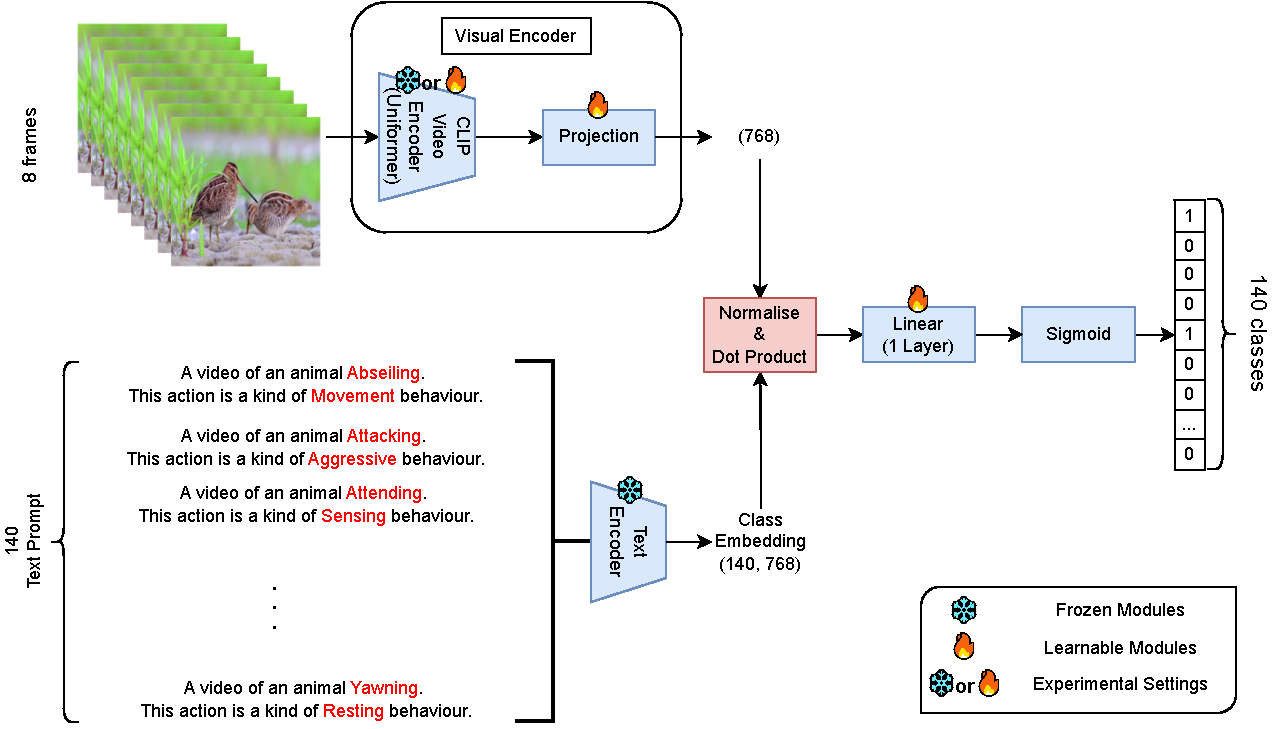
\includegraphics[width=1.0\textwidth]{assets/imgs/3_1_ModelStructureVC}
    \caption[VideoCLIP model structure]{This chart illustrates VideoCLIP model structure.}
    \label{fig:modelstructure_vc}
\end{figure}

\begin{figure}[ht]
    \centering
    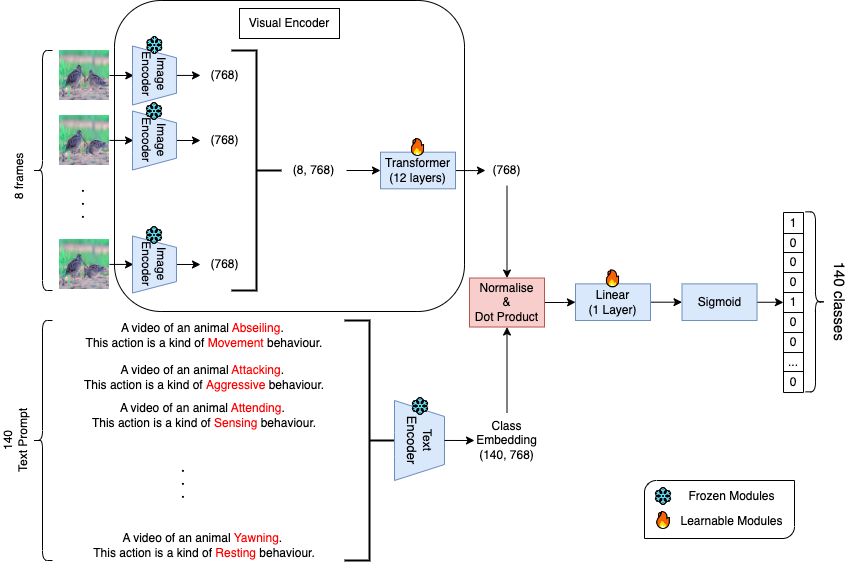
\includegraphics[width=1.0\textwidth]{assets/imgs/3_2_ModelStructureIC}
    \caption[ImageCLIP Model Structure]{This chart illustrates ImageCLIP model structure.}
    \label{fig:modelstructure_ic}
\end{figure}

Two model structures are employed for testing the performance of action recognition: 
\begin{enumerate}
    \item VideoCLIP: CLIP pretrained on videos, the clip module of InternVideo \parencite{wang2022internvideo} is used here. The whole structure is illustrated in Figure \ref{fig:modelstructure_vc}.
    \item ImageCLIP: CLIP pretrained on images, the original CLIP \parencite{radford2021learning} is used here. The whole model structure is illustrated in Figure \ref{fig:modelstructure_ic}.
\end{enumerate}

Both models utilise CLIP and prompt engineering for action recognition, taking videos and text prompts as input. The prompt template "A video of an animal
<action>. This action is a kind of <category of action> behaviour." is employed to generate the prompt for producing class embeddings. As shown in Figure \ref{fig:1_1_ClassEmbeddingInternVideo}, this method can produce meaningful distributed class embeddings.

Before training begins, in order to accelerate the process, the class embeddings of size $(140, 768)$ are pre-calculated by a text encoder pretrained by InternVideo based on the prompt template, action name, and category. This is done since the text encoder is frozen, and the weights are not updated. 

Figure \ref{fig:modelstructure_vc} shows the model structure of VideoCLIP. In order to evaluate the structure fairly, two model settings are experimented with on this structure: VideoCLIP training on all vision layers, and VideoCLIP training only on projection layers. Figure \ref{fig:modelstructure_ic} shows the model structure of ImageCLIP. In order to encode the 8 frames into video embeddings, 8 image embeddings encoded by the image encoder of ImageCLIP should be further passed through a 12-layer transformer followed by a pooling layer to produce a 768-dimensional video embedding.

As this is a multilabel classification task, meaning that a video may belong to more than one class, a linear layer is added as a buffer to help the model fit better. Finally, the output logits of the linear layer are then passed through a sigmoid function to determine the probability of each class. 

\section{AFRICAN}
The whole AFRICAN consists of two stages: the pretraining stage and the action recognition stage. The pretraining stage is to train the model to distinguish whether two images are augmented from the same frame in a video or not. At the action recognition stage, the pretrained AFRICAN image encoder is applied to extract the embeddings for action recognition. 

\subsection{Pretraining Stage}

\begin{figure}[ht]
    \centering
    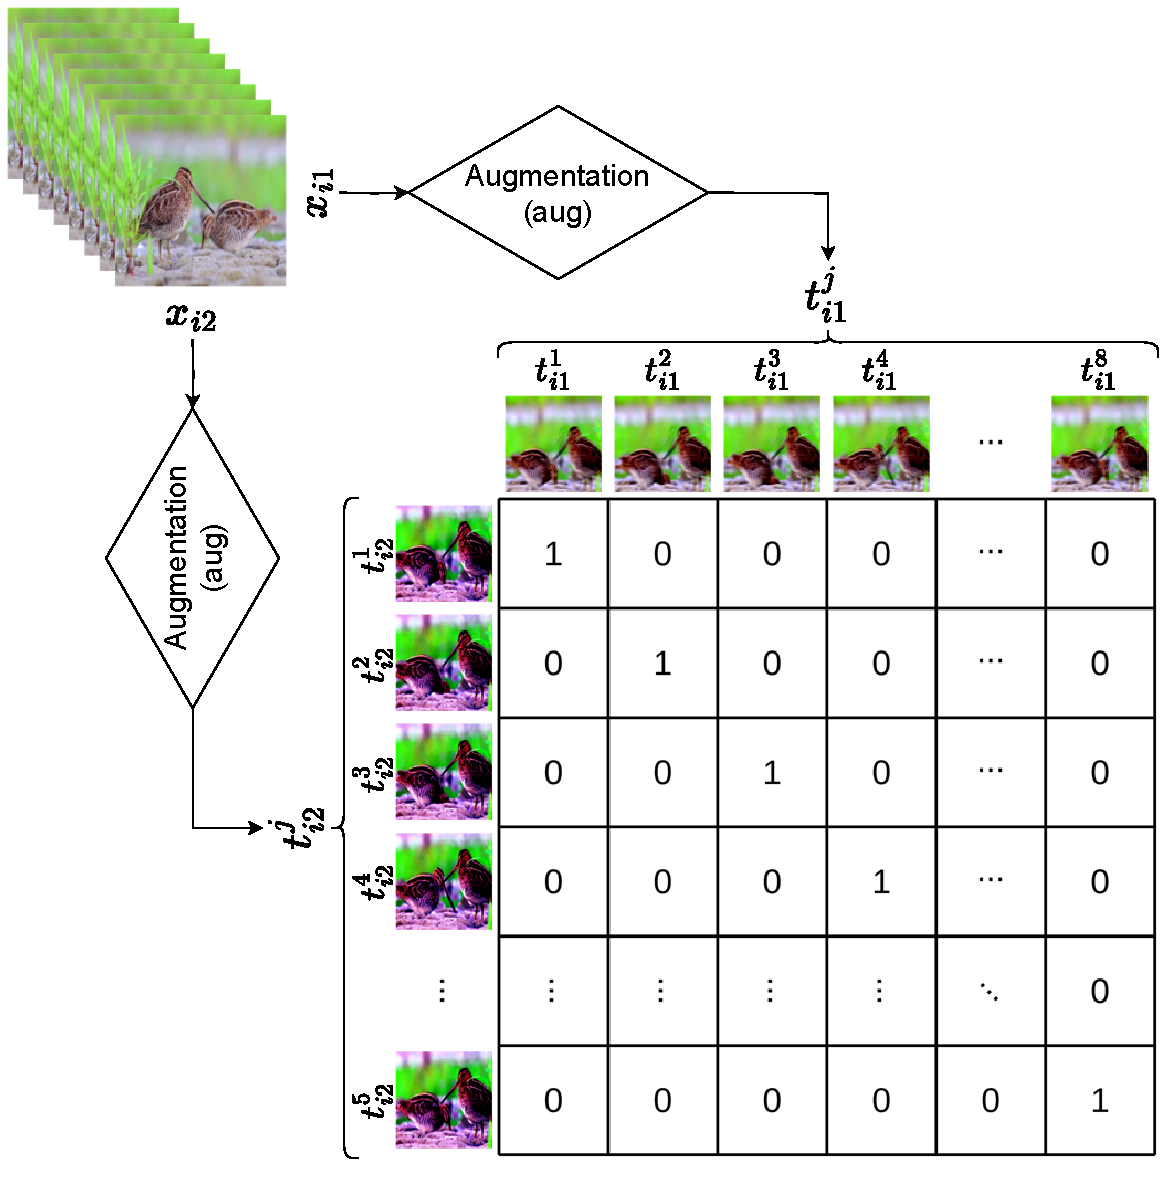
\includegraphics[width=0.6\textwidth]{assets/imgs/3_3_ConstrastiveSimilarityMatrix}
    \caption[Operation of pretraining AFRICAN]{This chart illustrates the operation of pretraining AFRICAN.}
f\label{fig:modelstructafsim}
\end{figure}

At the pretraining stage, AFRICAN applies contrastive learning techniques to distinguish whether two images are augmented from the same frame in a video or not. Figure \ref{fig:modelstructafsim} illustrates the batch operation of the model. The input for forwarding is a video sample $x_i$, where $i$ denotes the $i$-th sample in the dataset. $x_i$ is then copied twice into $x_{i1}$ and $x_{i2}$, which then independently pass through the same video augmentation function $aug(\cdot)$ with different random state, as shown in Equations \ref{eq:aug1} and \ref{eq:aug2}. 

\begin{equation}
    \label{eq:aug1}
    t_{i1} = aug(x_{i1})
\end{equation}
\begin{equation}
    \label{eq:aug2}
    t_{i2} = aug(x_{i2})
\end{equation}

After the transformation, $t_{i1}$ and $t_{i2}$ are separated into $j$ frames, denoted as $t_{i1}^j$ and $t_{i2}^j$. In this research, 8 frames are sampled from a video in a batch. Each frame will go through the same image encoder $f(\cdot)$ to be encoded into embeddings $e_{i1}^j$ and $e_{i2}^j$, as shown in Equations \ref{eq:enc1} and \ref{eq:enc2}.

\begin{equation}
    \label{eq:enc1}
    e_{i1}^j = f(t_{i1}^j)
\end{equation}
\begin{equation}
    \label{eq:enc2}
    e_{i2}^j = f(t_{i2}^j)
\end{equation}

Afterwards, the similarity between the image embeddings is calculated by normalisation and dot product, as shown in Equation \ref{eq:sim}, where $k$ denotes the frame index of $e_{i1}$ and $l$ denotes the frame index of $e_{i2}$. The numbers in the matrix in Figure \ref{fig:modelstructafsim} represent the learning targets for different image pair inputs. The diagonal line represents the frame pairs augmented from the same frames, while other numbers indicate pairs of images from different source frames. 

\begin{equation}
    \label{eq:sim}
    t_{i}^{kl} = norm(e_{i1}^{k}) \cdot norm(e_{i2}^{l})
\end{equation}




\subsection{Action Recognition Stage}

\begin{figure}[ht]
    \centering
    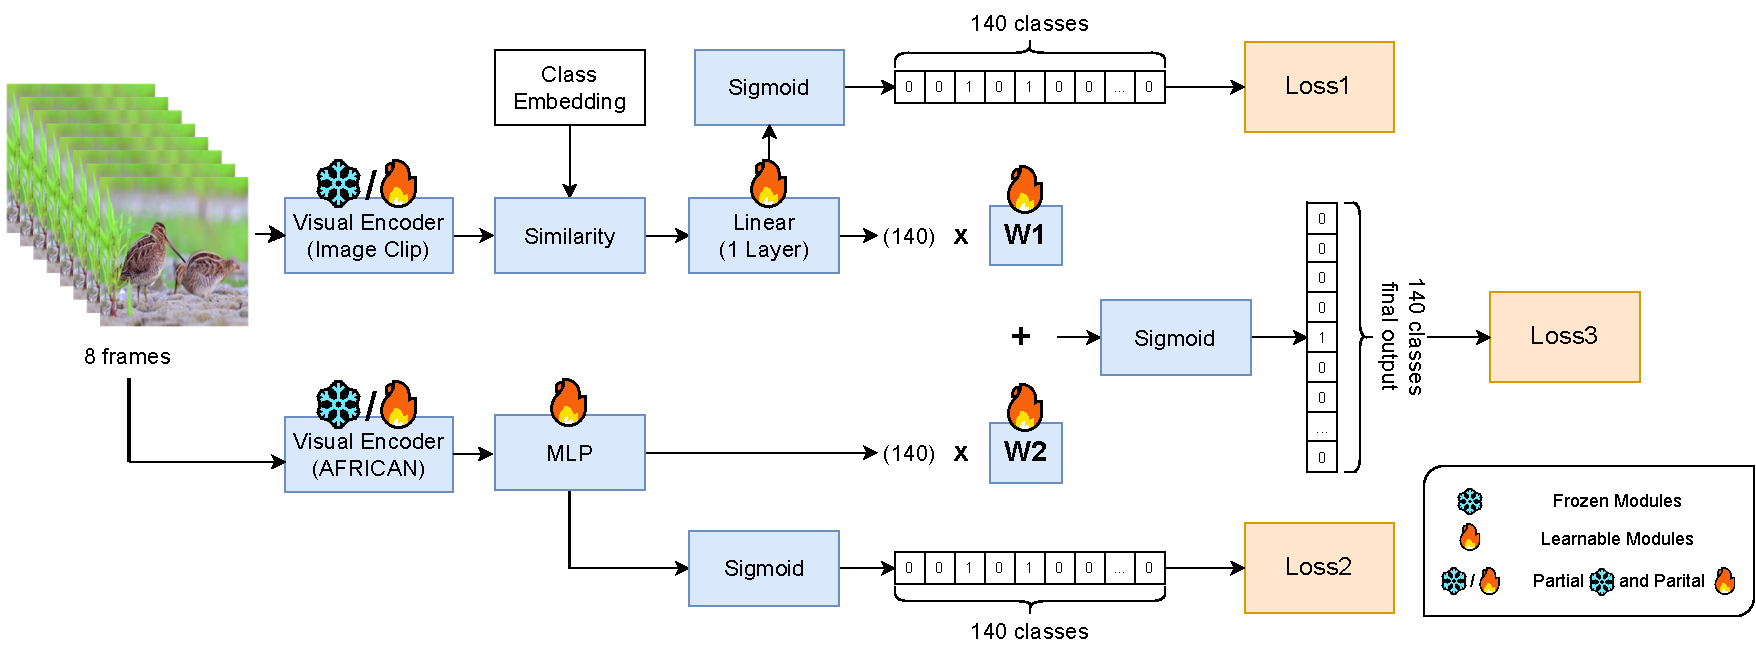
\includegraphics[width=1.0\textwidth]{assets/imgs/3_4_ModelStructureAF}
    \caption[Operation of AFRICAN for action recognition]{This chart illustrates the operation of AFRICAN for action recognition.}
    \label{fig:modelstructaf_ar}
\end{figure}

% TODO: further discussion is in the ablation study
Figure \ref{fig:modelstructaf_ar} illustrates the operation of AFRICAN for action recognition. The whole structure consists of two streams. The upper stream is the pretrained CLIP stream, the lower stream is the pretrained AFRICAN stream. 

In the pretrained CLIP stream, the visual encoder and class embedding are the same as those in ImageCLIP, as shown in Figure \ref{fig:modelstructure_ic}. Because the structure of ImageCLIP is able to achieve better performance than VideoCLIP, which will be discussed in Section \ref{sec:imageclipbetter}, ImageCLIP is employed here as the visual encoder in the pretrained CLIP stream. 

In the pretrained AFRICAN stream, the structure of the visual encoder is the same as those in the pretrained CLIP stream but with AFRICAN pretrained weights. Since AFRICAN is not pretrained by the vision-text multimodal model like CLIP, there is no corresponding class embedding. Therefore, a commonly used structure, the multilayer perceptron (MLP), is employed to map the embedding and one-hot encoding. The 3-layer MLP takes the video embedding as input and outputs 140-dimensional logits, which are then passed through a sigmoid function for classification.

After the logits, the input of the sigmoid function, are obtained in the two streams, they are used separately for prediction and computation of loss1 and loss2. Simultaneously, the logits of both streams are multiplied by W1 and W2, two 140-dimensional weights, respectively to determine the contributions of each class for both streams. This is followed by an addition to produce the final prediction and computation of loss3. Finally, loss1, loss2, and loss3 are added together to do the backpropagation. 
